\documentclass[border=3pt]{standalone}
\usepackage{tikz}
\usepackage{amsmath}
\usepackage{amssymb}
\usepackage{ctex}
\usetikzlibrary{matrix, calc, positioning}
\usepackage{pgfplots}
\pgfplotsset{compat=1.18}

\begin{document}
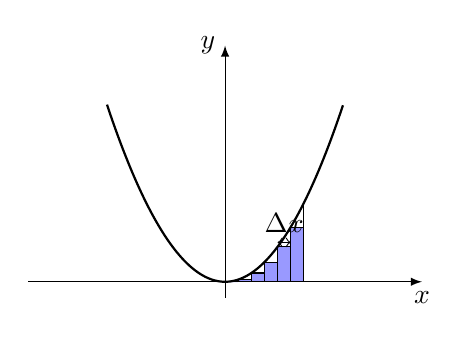
\begin{tikzpicture}[declare function={f(\x)=(\x)^(2);},
		lnode/.style={fill=white,font=\small,inner sep=0pt}]
	\providecommand*{\N}{6}
	\renewcommand*{\N}{6}
	\pgfmathtruncatemacro{\M}{\N/4}
	\coordinate (start) at (0,{f(0)});
	\foreach \X [remember=\X as \LastX (initially 0)] in {1,...,\N}
		{
			\draw[fill=blue!40!white] (\LastX/\N,0) rectangle (\X/\N,{f(\LastX/\N)});
			% \draw[red,fill=red] (1+\LastX*4/\N,{f(1+\LastX*4/\N)}) circle (2pt) ;
			\path  (\LastX/\N,0pt) coordinate (x\X);
		}
	\coordinate (end) at (1,{f(1)});
	\draw (1,0)--(1,{f(1)});
	\draw [-latex] (-2.5,0) -- (2.5,0) node (xaxis) [below] {$x$};
	\draw [-latex] (0,-0.2) -- (0,3) node [left] {$y$};
	\draw[domain=-1.5:1.5,samples=200,variable=\x,-,thick] plot ({\x},{f(\x)});
	\draw[<->] (x5|- 0,1/2)--(x6|- 0,1/2) node[above, midway] {$\Delta x$};
\end{tikzpicture}

\end{document}
